\rev{\section{Preliminary User study}
\label{sec:user_study}
In addition to validating the effectiveness of \modelname, this section presents the feedbacks of users on the design and user experience of \sysname.

\subsection{Procedure}
We distributed a semi-structured questionnaire to the 112 participants in \secref{sec:eval}.
All the participants were paid about 20 USD (in the local currency) after the survey.
We present the main results as follows\footnote{Not that most participants are not proficient in English. The original questionnaire was in the mouth tongue of the participants. The responses were carefully translated into English and presented in the results.}.

\subsection{Results}

\subsubsection{Operability of \sysname}
In this part of the survey, the participants were asked to rate the overall operability of \sysname as well as the three manual operations (food, drug and insulin intake) with three levels (\textit{Inconvenient}, \textit{Normal} and \textit{Convenient}).
The participants make comments on their practical operations. For example, the non-diabetic users who do not need to record drugs and insulin only rate the operation of food input, and the diabetic users who do not inject insulin are only report their comments on the food and drug inputs.
They were also required to express their opinions on the overall operability.

\begin{figure}[h]
  \centering
  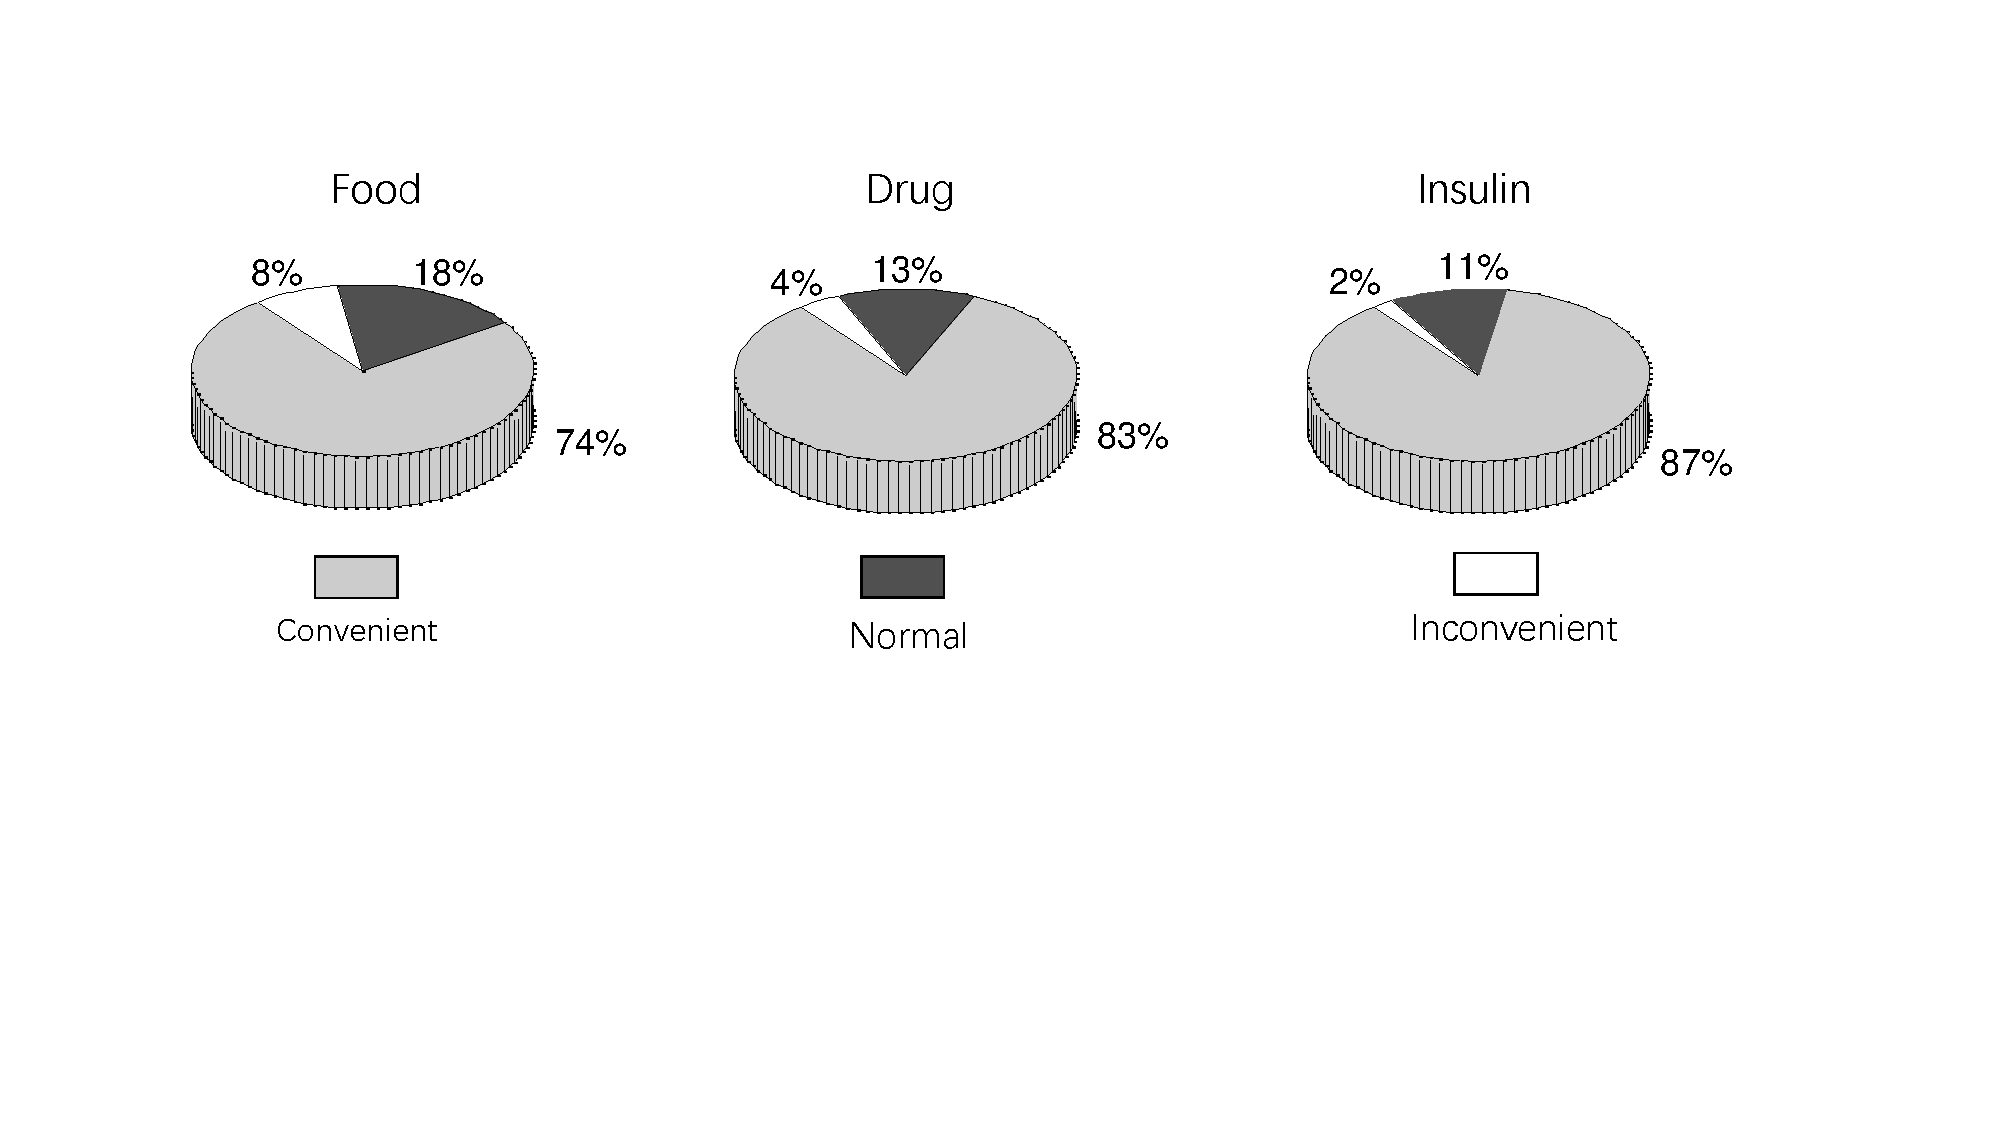
\includegraphics[width=0.8\columnwidth]{./img/user_cases.pdf}
  \caption{\rev{Distributions of user rating on the operability of food, drug and insulin intake recording interfaces.}}
  \label{fig:user_cases}
\end{figure}

\figref{fig:user_cases} illustrates the distributions of the user ratings on the operability of food, drug and insulin intake recording interfaces.
The lowest rates are seen for manual recording of food intake (74\% as \textit{Convenient}).
The ratings for manual recording of drug and insulin intake are slightly better.
Overall, 78\%, 18\% and 4\% of the participants rate \sysname as \textit{Convenient}, \textit{Normal} and \textit{Inconvenient}, respectively.
%\TODO{present the results for the three groups of users separately, because non-diabetic users may not need to record drug and insulin intake, which leads them to give a higher rank.}

We select one representative comment for each level as follows:
\begin{itemize}
  \item
  \textit{``This App is easy to learn and quick to use.
  The database of food, drugs and insulin is very comprehensive.''}
  [Convenient, Type II diabetic user]
  \item
  \textit{``What I would like to see is a way to fill in the daily inputs by taking photos and speaking to.
  It would be more convenient to operate.''}
  [Normal, Type I diabetic user]
  \item
  \textit{``I don't have much time to record what I had for each meal using a scrolling menu.
  The App should be more personalized.
  For example, it should learn from my input history and provide search hints or automatic records.''}
  [Inconvenient, non-diabetic user]
\end{itemize}

As expected, the manual recording of food, drug and insulin intake tends to be a burden for \sysname as an intriguing application.
Nevertheless, we have collected some constructive suggestions from the users.
For instance, speech input instead of a scrolling menu might be a more welcome input mechanism.
Intelligent search hints based on personal input history using recommendation algorithms~\cite{bib:fu2000mining} may help to improve the user experience when recording food intake, which is highly diversified and challenging to record automatically.

\subsubsection{Benefits of \sysname}
In this part of the survey, each participant is asked to comment whether \sysname is useful by rating \sysname in three levels (\textit{Instructive}, \textit{Normal} and \textit{Non-instructive}) and commenting in detail.

94\% of the participants report \sysname as \textit{Instructive} and 6\% report \textit{Normal}.
No participant rates \sysname as \textit{Non-instructive}.
We also list two representative comments below.
\begin{itemize}
  \item
  \textit{``\sysname guides me to control my blood glucose and helps to live a healthier lifestyle.
  For instance, I always observe the blood glucose dynamics after meals.
  \sysname helps to figure out that my blood glucose rises a lot after I eat noodles, breads and dumplings, but stays relatively stable after eating meats and vegetables.
  Also I can learn about the impact of the drugs on my blood glucose.
  I'm happy to understand how my lifestyle affects my blood glucose and learn to make some adjustments in time.
  I have recommended \sysname to six friends.
  They also care about their blood glucose levels.''}
  [Instructive, Type II diabetic user]
  \item
  \textit{``I'm not diabetic but I feel I need to start tracking my blood glucose occasionally.
  This app has made it easy but still has room to improve.
  It presents me a short-term impact of food intake.
  However, I still care about how to maintain a long-term healthy status.
  Specifically, it should provide some suggestions to help me prevent developing into diabetes.''}
  [Normal, non-diabetic user]
\end{itemize}
In summary, users expect more functionalities of \sysname such as recommending intensity and time of exercises and recommending food plans.
In this regard, the personalized blood glucose dynamics records collected by \sysname can be sent to the experts to recommend personalized precautionary measures.

\subsubsection{Willingness to use \sysname}
Finally, we are interested in whether the participants are willing to use \sysname for blood glucose tracking despite the manual input of food, drug and insulin intake.
In the questionnaire, we ask the following question:
\textit{``Are you willing to use \sysname instead of the CGM device at cost of manual recording of daily food, drug and insulin intake, as well as the periodic CGM re-calibration once every two or three weeks ?''}
We also collect free-response comments as before.
\begin{figure}[h]
  \centering
  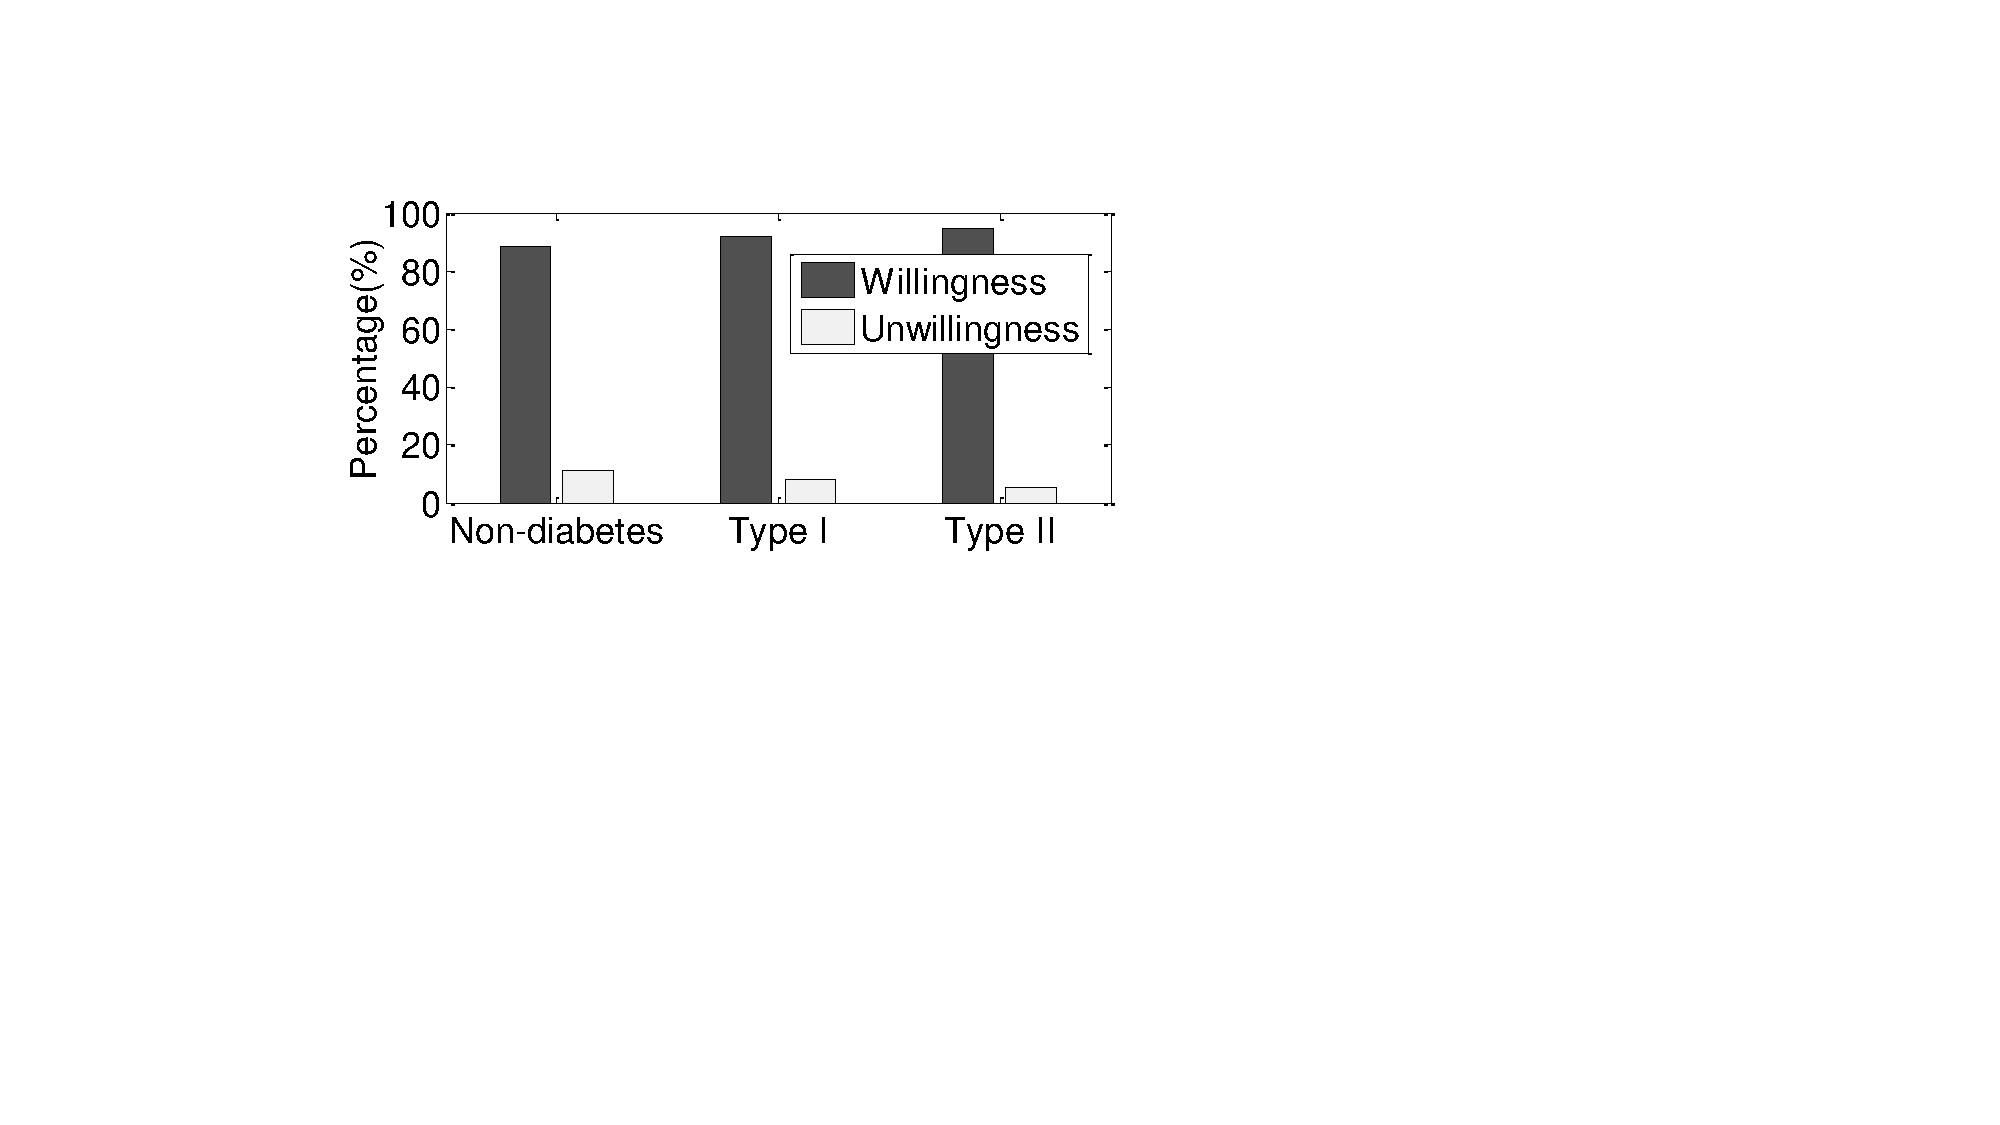
\includegraphics[width=0.4\columnwidth]{./img/willingness.pdf}
  \caption{\rev{Willingness to use \sysname.}}
  \label{fig:user_willingness}
\end{figure}

\figref{fig:user_willingness} illustrates the results.
Over 90\% diabetic users (both Type I and Type II) are willing to use \sysname while non-diabetic users show a slightly lower willingness (85\%).
We also select two representative comments.
\begin{itemize}
  \item
  \textit{``
  Manual records seem much more convenient compared to wearing the CGM.
  I feel very uncomfortable when wearing the CGM.
  It reminds me that I am a patient all the time.
  Wearing the CGM device for calibration once a month is acceptable.
  At least 3/4 of the time I am free from the CGM device.''}
  [Willing, Type II diabetic user]
  \item
  \textit{``
  I am OK with the periodic CGM calibration, but the daily food recording is a pain for me.
  I always eat outside and easily forget what I have had after the meal.
  I'm not a patient.
  I don't like to record everything I did simply to track my blood glucose.''}
  [Unwilling, non-diabetic user]
\end{itemize}
From the feedbacks, it seems that most participants feel that continuous wearing of CGM devices is more uncomfortable.
Even if periodic re-calibration is required, many diabetic users think it is acceptable.
The manual recording of food intake is again the major concern, especially among non-diabetic participants. We will optimize the food recording function in our future work.




}
